%%%%%%%%%%%%%%%%%%%%%%%%%%%%%%%%%%%%%%%%%%%%%%%%%%%
%																													
%																												
%																													
%									Importations	de bibliothèques	
%																													
%																												
%%%%%%%%%%%%%%%%%%%%%%%%%%%%%%%%%%%%%%%%%%%%%%%%%%%


\documentclass[hidelinks]{article}
\usepackage[utf8]{inputenc}
\usepackage{graphicx}
\usepackage[T1]{fontenc}
\usepackage[french]{babel}
\usepackage{csquotes}
\usepackage[section]{placeins}
\usepackage{tikz}
\usepackage{hyperref}
\usepackage{afterpage}
\usepackage{pdfpages}
\usepackage{wrapfig}
\usepackage{amsmath, mathtools}
\usepackage{amssymb}
\usepackage{fancyhdr}
\usepackage[all]{background}


%%%%%%%%%%%%%%%%%%%%%%%%%%%%%%%%%%%%%%%%%%%%%%%%%%%%%%%%%%%%%%%%%%%%
%																																	   %
%																																	   %
%																																	   %
%															Page de garde															   %
%																																	   %
%																																	   %
%%%%%%%%%%%%%%%%%%%%%%%%%%%%%%%%%%%%%%%%%%%%%%%%%%%%%%%%%%%%%%%%%%%%



\newcommand{\MyGraphicLogo}{% For imported graphic logo
\begin{tikzpicture}[remember picture,overlay,yshift=-15cm, xshift=10.5cm]
	\definecolor{gris}{RGB}{16,52,78}
	\definecolor{jaune_fonce}{RGB}{0, 107, 163}
	\definecolor{jaune}{RGB}{0, 151, 136}
	\fill [gris] (-10.5,-10) -- (0,-4.5) -- (14,-13) -- (14,-16)--(0,-16)--(-10.5,-16);
	\fill [jaune_fonce] (0,-4.5) -- (-10.5,-10) -- (-10.5, 1.8);
	\node at (3.8,0.4) {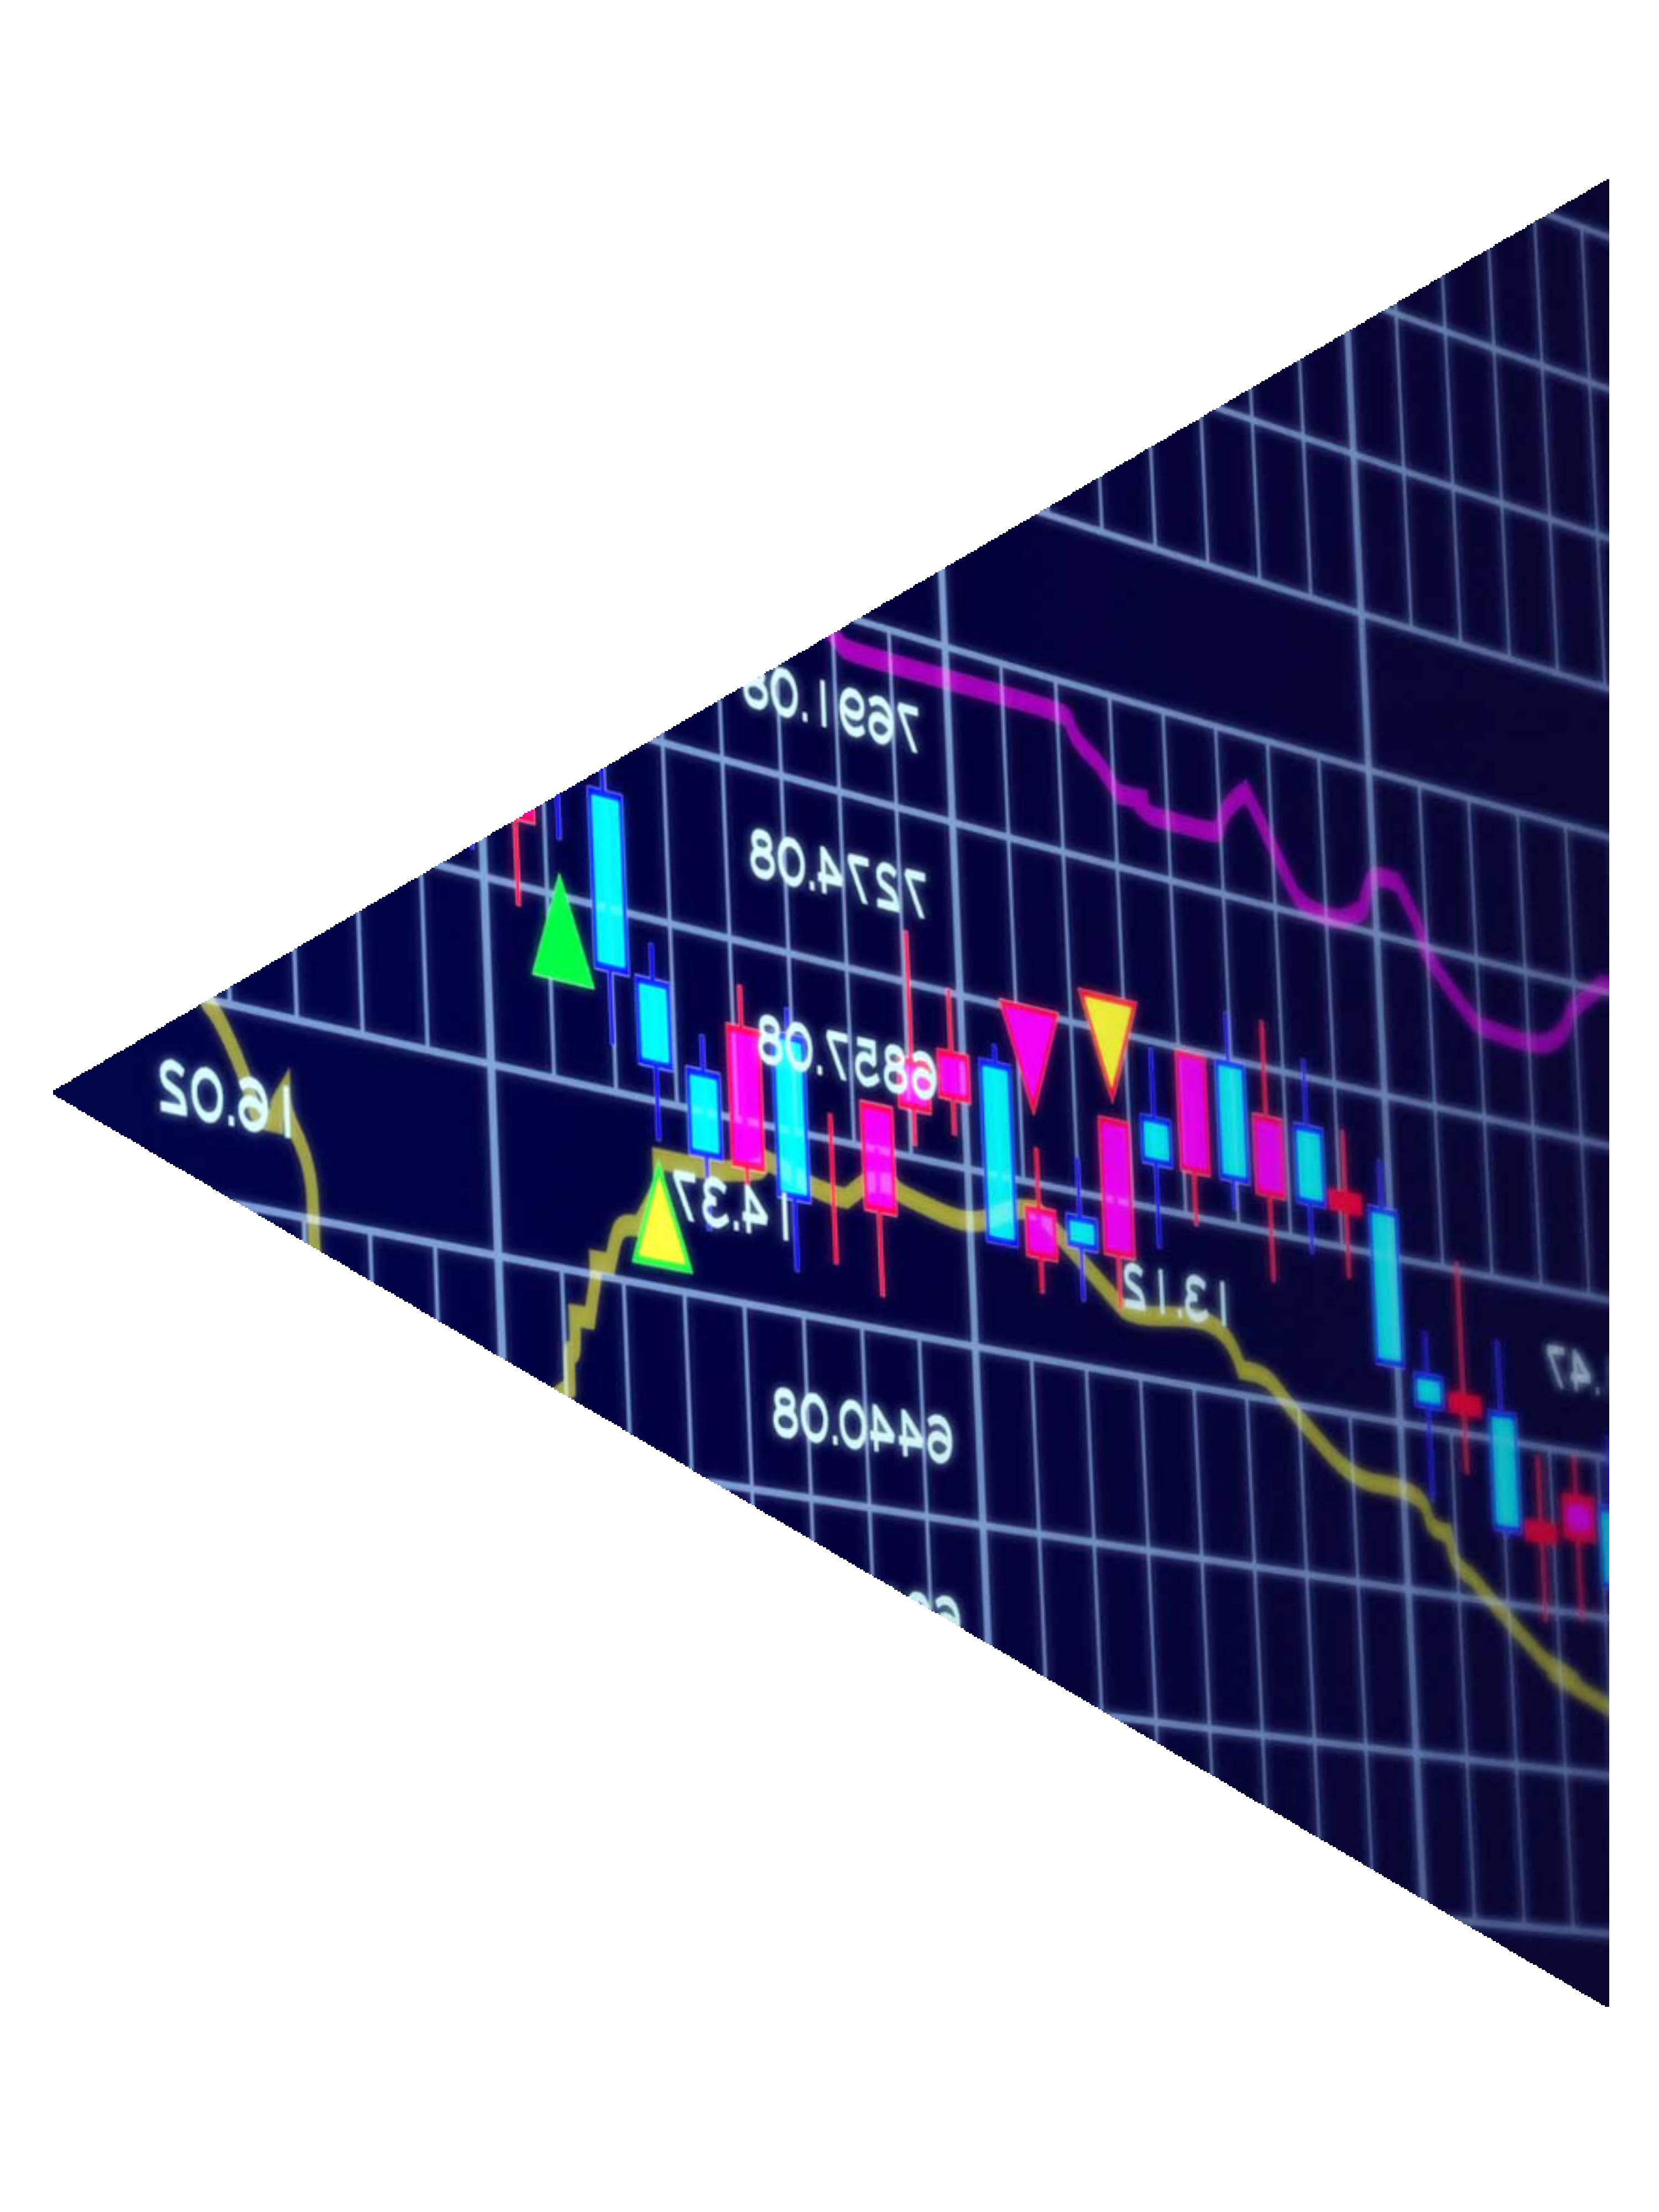
\includegraphics[width=22cm]{triangle.png}};
	\fill [jaune] (14,5) -- (2.5, 12) -- (20,25) -- (14, 20);
 \end{tikzpicture}}


\SetBgContents{\MyGraphicLogo}% Select included image

\SetBgPosition{current page.north west}% Select location
\SetBgOpacity{1.0}% Select opacity
\SetBgAngle{0.0}% Select roation of logo
\SetBgScale{1.0}% Select scale factor of logo



%%%%%%%%%%%%%%%%%%%%%%%%%%%%%%%%%%%%%%%%%%%%%%%%%%%%%%%%%%%%%%%%%%%%
%																																	   %
%																																	   %
%																																	   %
%										Informations générales sur le document															   %
%																																	   %
%																																	   %
%%%%%%%%%%%%%%%%%%%%%%%%%%%%%%%%%%%%%%%%%%%%%%%%%%%%%%%%%%%%%%%%%%%%

 \usepackage{fontspec}
  \usepackage[bold-style=upright]{unicode-math}
  \defaultfontfeatures{Scale=1}
  \setmainfont[Ligatures=TeX,Numbers=OldStyle]{Lucida Bright OT}
  \setmathfont[RawFeature=+ss04]{Lucida Bright Math OT}
  \setsansfont[Scale=1.0,Numbers=OldStyle]{Myriad Pro}
  \newfontfamily\fullcaps[Letters=Uppercase,Numbers=Uppercase]{Myriad Pro}
  \usepackage[babel=true]{microtype}
  \usepackage{icomma}
  
  
  
  
  
  
  
  
  
  
  
\title{Taylor series}
\author{Maxence COUPET - \href{mailto:maxence.coupet@gmail.com}{maxence.coupet@gmail.com}}
\date{March 2018}



\MHInternalSyntaxOn
\MH_set_boolean_T:n {outer_mult}
\MHInternalSyntaxOff

\newenvironment{nalign}{
    \begin{equation}
    \begin{aligned}
}{
    \end{aligned}
    \end{equation}
    \ignorespacesafterend
}
%%%%%%%%%%%%%%%%%%%%%%%%%%%%%%%%%%%%%%%%%%%%%%%%%%%%%%%%%%%%%%%%%%%%
%																																	   %
%																																	   %
%																																	   %
%												Mis en page du document																   %
%																																	   %
%																																	   %
%%%%%%%%%%%%%%%%%%%%%%%%%%%%%%%%%%%%%%%%%%%%%%%%%%%%%%%%%%%%%%%%%%%%


\begin{document}
	\selectlanguage{french}
	% page de garde
	\pagenumbering{gobble}
	\maketitle
	\newpage
	% début du rapport
	
	
	


\newcommand{\MyGraphicLog}{% For imported graphic logo
\begin{tikzpicture}[remember picture,overlay,yshift=-15cm, xshift=10.5cm]
\definecolor{jaune}{RGB}{16, 52, 78};
\fill[jaune] (-11, -16) -- (13, -16) -- (13, -12.1) -- (-11, -12.1);
 \end{tikzpicture}}


\SetBgContents{\MyGraphicLog}% Select included image


\SetBgPosition{current page.north west}% Select location
\SetBgOpacity{1.0}% Select opacity
\SetBgAngle{0.0}% Select roation of logo
\SetBgScale{1.0}% Select scale factor of logo

\pagestyle{fancy}
\renewcommand\headrulewidth{0pt}
\lhead{}\chead{}\rhead{}
\cfoot{\vspace*{6\baselineskip} \textcolor{white}{\thepage} \large}
	\newpage

	\pagenumbering{arabic}

%%%%%%%%%%%%%%%%%%%%%%%%%%%%%%%%%%%%%%%%%%%%%%%%%%%%%%%%%%%%%%%%%%%%
%																																	   %
%																																	   %
%																																	   %
%								Début du document (commencez à taper votre texte ici)													   %
%																																	   %
%																																	   %
%%%%%%%%%%%%%%%%%%%%%%%%%%%%%%%%%%%%%%%%%%%%%%%%%%%%%%%%%%%%%%%%%%%%

	\section{Taylor's theorem}
	
	Let $I$ be an interval, $a \in I$ and $f$ a function which is $n>1$ times derivable.
    \begin{nalign}
    \forall x \in I, \quad f(x) &= \begin{multlined}[t]f(a) + \frac{f'(a)}{1!}(x-a)+\frac{f^{(2)}(a)}{2!}(x-a)^{2}+\dots+ \\ 
    \frac{f^{(n)}(a)}{n!}(x-a)^{n}+R_{n}(x) \end{multlined} \\
    &= \sum_{k=0}^{n}\frac{f^{(k)}(a)}{k!}(x-a)^{k}+R_{n}(x)
    \end{nalign}

	By using a change of variable, we also have :
	\begin{nalign}
     f(a+h) &= \begin{multlined}[t]f(a) + \frac{h}{1!}f'(a)+\frac{h^2}{2!}f^{(2)}(a)+\dots+ \\ 
    \frac{h^n}{n!}f^{(n)}(a)+R_{n}(h) \end{multlined} \\
    &= \sum_{k=0}^{n} \frac{h^k}{k!}f^{(k)}(a)+R_{n}(h)
    \end{nalign}
    \newpage
    \section{Usual functions}
    
    \subsection{Exponential}
    
    \begin{nalign}
    \forall x \in \mathbb{R}, \quad e^x &= 1 + x + \frac{x^2}{2!} + \frac{x^3}{3!} + \dots \\
    &= \sum_{n=0}^{\infty}\frac{x^n}{n!}
    \end{nalign}
    
    \subsection{Logarithm}
    
    
    
     \begin{nalign}
    \forall x \in ]-1,1[, \quad ln(1-x) &= - x - \frac{x^2}{2} - \frac{x^3}{3} - \dots \\
    &=- \sum_{n=1}^{\infty}\frac{x^n}{n}
    \end{nalign}
    
     \begin{nalign}
    \forall x \in ]-1,1[, \quad ln(1+x) &= x - \frac{x^2}{2} + \frac{x^3}{3} - \dots \\
    &=\sum_{n=1}^{\infty}(-1)^{n+1}\frac{x^n}{n}
    \end{nalign}
    
    
    \subsection{Geometric series}
    
    \begin{nalign}
    \forall x \in ]-1,1[, \quad \frac{1}{1-x} &= 1 + x + x^2 + x^3 + \dots \\
    &=\sum_{n=0}^{\infty}x^n
    \end{nalign}
    
    \begin{nalign}
    \forall x \in ]-1,1[, \quad \frac{1}{(1-x)^2} &= 1 +2 x + 3x^2 + 4x^3 + \dots \\
    &=\sum_{n=1}^{\infty}nx^{n-1}
    \end{nalign}
    
    \begin{nalign}
    \forall x \in ]-1,1[, \quad \frac{1}{(1-x)^3} &= 1 +3 x + 4x^2 + 10x^3 + \dots \\
    &=\sum_{n=2}^{\infty}\frac{(n-1)n}{2}x^{n-2}
    \end{nalign}
    
    \subsection{Binomial series}
    
    \begin{nalign}
    \forall x \in ]-1,1[, \quad (1-x)^\alpha &= \begin{multlined}[t]1 +\alpha x + \frac{\alpha(\alpha - 1)}{2!} x^2 \\ + \frac{\alpha(\alpha - 1)(\alpha - 2)}{3!}x^3 + \dots \end{multlined}\\
    &=\sum_{n=0}^{\infty}\left( \prod_{k=1}^{n}\frac{\alpha-k-1}{k} \right)x^n
    \\ & = \sum_{n=0}^{\infty} \binom{\alpha}{n}x^n
    \end{nalign}
    
    Two particular values of $\alpha$ are interesting : $\alpha=\frac{1}{2}$ and $\alpha=-\frac{1}{2}$ , which gives use the square root function and its inverse : 
    \begin{nalign}
    \forall x \in ]-1,1[, \quad \sqrt{1-x} &= 1 + \frac{1}{2}x - \frac{1}{8}x^2 + \frac{1}{16}x^3- \dots
    \end{nalign}
    
    \begin{nalign}
    \forall x \in ]-1,1[, \quad \frac{1}{\sqrt{1-x}} &= 1 - \frac{1}{2}x + \frac{3}{8}x^2 - \frac{5}{16}x^3+ \dots
    \end{nalign}
    
    \subsection{Trigonometric functions}
    
    \begin{nalign}
    \forall x \in \mathbb{R}, \quad sin(x) &= x - \frac{x^3}{6} + \frac{x^5}{120} - \dots \\
    &= \sum_{n=0}^{\infty}\frac{(-1)^n}{(2n+1)!}x^{2n+1}
    \end{nalign}
    
     \begin{nalign}
    \forall x \in \mathbb{R}, \quad cos(x) &= 1 - \frac{x^2}{2} + \frac{x^4}{24} - \dots \\
    &= \sum_{n=0}^{\infty}\frac{(-1)^n}{(2n)!}x^{2n}
    \end{nalign}
    
    \begin{nalign}
    \forall x \in \left]-\frac{\Pi}{2},\frac{\Pi}{2}\right[, \quad tan(x) &= x + \frac{x^3}{3} + \frac{2x^5}{15} + \dots
    \end{nalign}
    
    \begin{nalign}
    \forall x \in ]-1,1[, \quad arcsin(x) &= x + \frac{x^3}{6} + \frac{3x^5}{40} + \dots \\
    &= \sum_{n=0}^{\infty}\frac{(2n)!}{4^n (n!)^2 (2n+1)}x^{2n+1}
    \end{nalign}
    
    \begin{nalign}
    \forall x \in ]-1,1[, \quad arccos(x) &= \frac{\Pi}{2} - arcsin(x) \\
    & = \frac{\Pi}{2} - x - \frac{x^3}{6} - \frac{3x^5}{40} - \dots \\
    &= \frac{\Pi}{2} - \sum_{n=0}^{\infty}\frac{(2n)!}{4^n (n!)^2 (2n+1)}x^{2n+1}
    \end{nalign}
    
    \begin{nalign}
    \forall x \in ]-1,1[, \quad arctan(x) &= x - \frac{x^3}{3} + \frac{x^5}{5} - \dots \\
    &= \sum_{n=0}^{\infty}\frac{(-1)^n}{2n+1}x^{2n+1}
    \end{nalign}
    
    \subsection{Hyperbolic functions}
    
    \begin{nalign}
    \forall x \in \mathbb{R}, \quad sinh(x) &= x + \frac{x^3}{3!} + \frac{x^5}{5!} + \dots \\
    &= \sum_{n=0}^{\infty}\frac{x^{2n+1}}{(2n+1)!}
    \end{nalign}
    
    \begin{nalign}
    \forall x \in \mathbb{R}, \quad cosh(x) &= 1 + \frac{x^2}{2!} + \frac{x^4}{4!} + \dots \\
    &= \sum_{n=0}^{\infty}\frac{x^{2n}}{(2n)!}
    \end{nalign}
    
    \begin{nalign}
    \forall x \in \mathbb{R}, \quad tanh(x) &= x - \frac{x^3}{3} + \frac{2x^5}{15} - \dots 
    \end{nalign}
\end{document}